\begin{frame}[c]
  \frametitle{Case II : Vertical Advective Velocity and Diffusion Coefficient}
Advection is transport driven by bulk water velocity while diffusion is the 
result of Brownian motion across concentration gradients.  The method by which 
the dominant solute transport mode (diffusive or advective) is determined for a 
particular porous medium is by use of the dimensionless Peclet number, 

\begin{align} 
  Pe &= \frac{nvL}{\alpha nv + D_{eff}},\\
  &= \frac{\mbox{advective rate}}{\mbox{diffusive rate}}\nonumber
  \intertext{where} 
  n &= \mbox{ solute accessible porosity } [\%]\nonumber\\
  v &= \mbox{ advective velocity } [m\cdot s^{-1}] \nonumber\\
  L &= \mbox{ transport distance } [m]\nonumber\\
  \alpha &= \mbox{ dispersivity } [m]\nonumber\\
  D_{eff} &= \mbox{ effective diffusion coefficient } [m^2\cdot s^{-1}].\nonumber
\end{align}
For a high $Pe$ number, advection is the dominant transport mode, while 
diffusive or dispersive transport dominates for a low $Pe$ number
\cite{schwartz_fundamentals_2004}.
\end{frame}

\begin{frame}[c]
  \frametitle{Case II : Vertical Advective Velocity and Diffusion Coefficient}
  \begin{table}[ht!]
\centering
\footnotesize{
\begin{tabular}{|l|l|l|r|r|}
\multicolumn{5}{c}{\textbf{Simulation Cases}}\\
\hline
\textbf{Case} & \textbf{Parameter} & \textbf{Units} & \textbf{Min. Value} & \textbf{Max. Value}\\
\hline
II    & $V_{adv, y}$ & $[m \cdot yr^{-1}]$       & $6.31\times10^{-8}$  &  $6.31\times10^{-4}$ \\
      & $D_{eff}$    & $[m^2\cdot s^{-1}]$       & $10^{-8}$    &  $10^{-5}$ \\
\hline
\end{tabular}
\caption{Case II varied the advective velocity and effective diffusivity to 
  determine the nature of the threshold between the diffusive and advective 
  regimes. This dual parameter simulation case had 40 simulation 
groups of 100 realizations each.}
\label{tab:Cases}
}
\end{table}



The forty runs are a combination of the five values of the vertical advective 
velocity and eight magnitudes of relative diffusivity.
\begin{table}
\centering
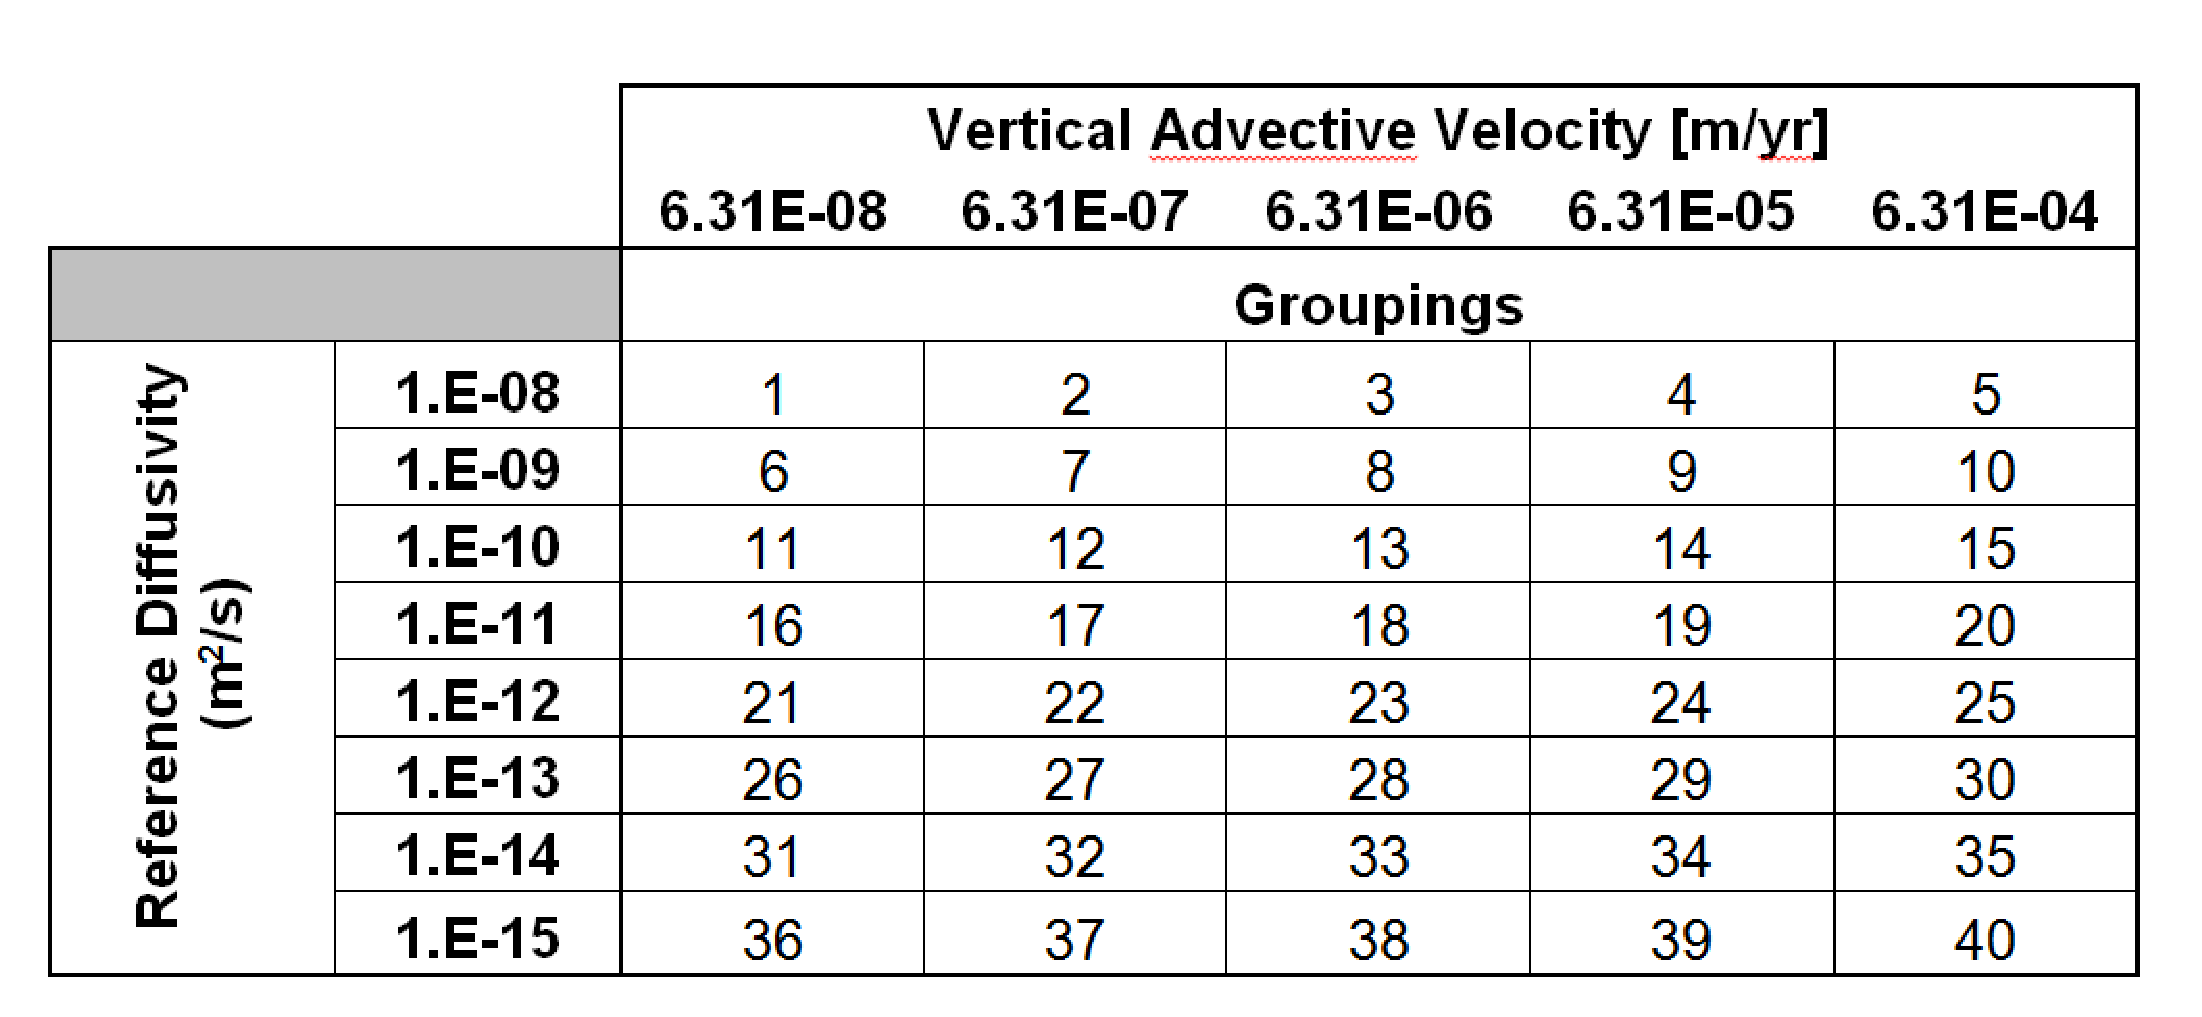
\includegraphics[width=0.8\textwidth]{AdvVelAndDiffCoeffEBSFail/AdvVelAndDiffCoeffGroups.eps}
\caption{Vertical advective velocity and diffusion coefficient simulation groupings.}
\label{tab:AdvVelAndDiffCoeffGroups}
\end{table}
\end{frame}

\begin{frame}[c]
  \frametitle{Case II : Vertical Advective Velocity and Diffusion Coefficient}
\begin{figure}[htp!]
\centering
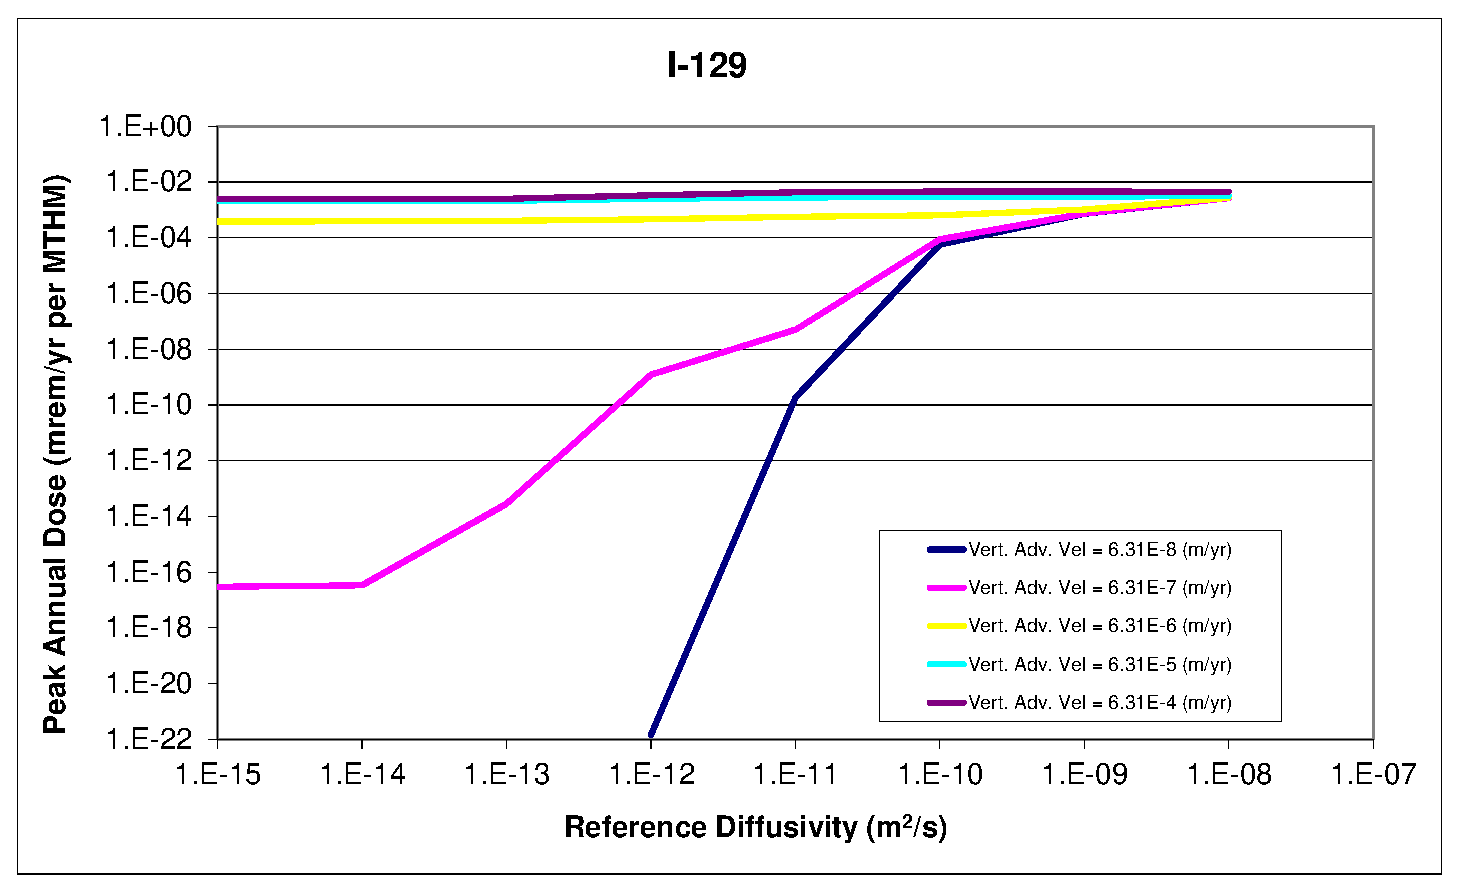
\includegraphics[width=0.8\textwidth]{AdvVelAndDiffCoeffEBSFail/I-129.eps}
\caption{$^{129}I$. For vertical advective velocities 
$6.31\times10^{-6}[m/yr]$ and above, lower reference diffusivities are 
ineffective at attenuating the mean of the peak doses for soluble, non-sorbing 
elements. 
}
\label{fig:VAdvVelI129}
\end{figure}
\end{frame}

\begin{frame}[c]
  \frametitle{Case II : Vertical Advective Velocity and Diffusion Coefficient}
\begin{figure}[htp!]
\centering
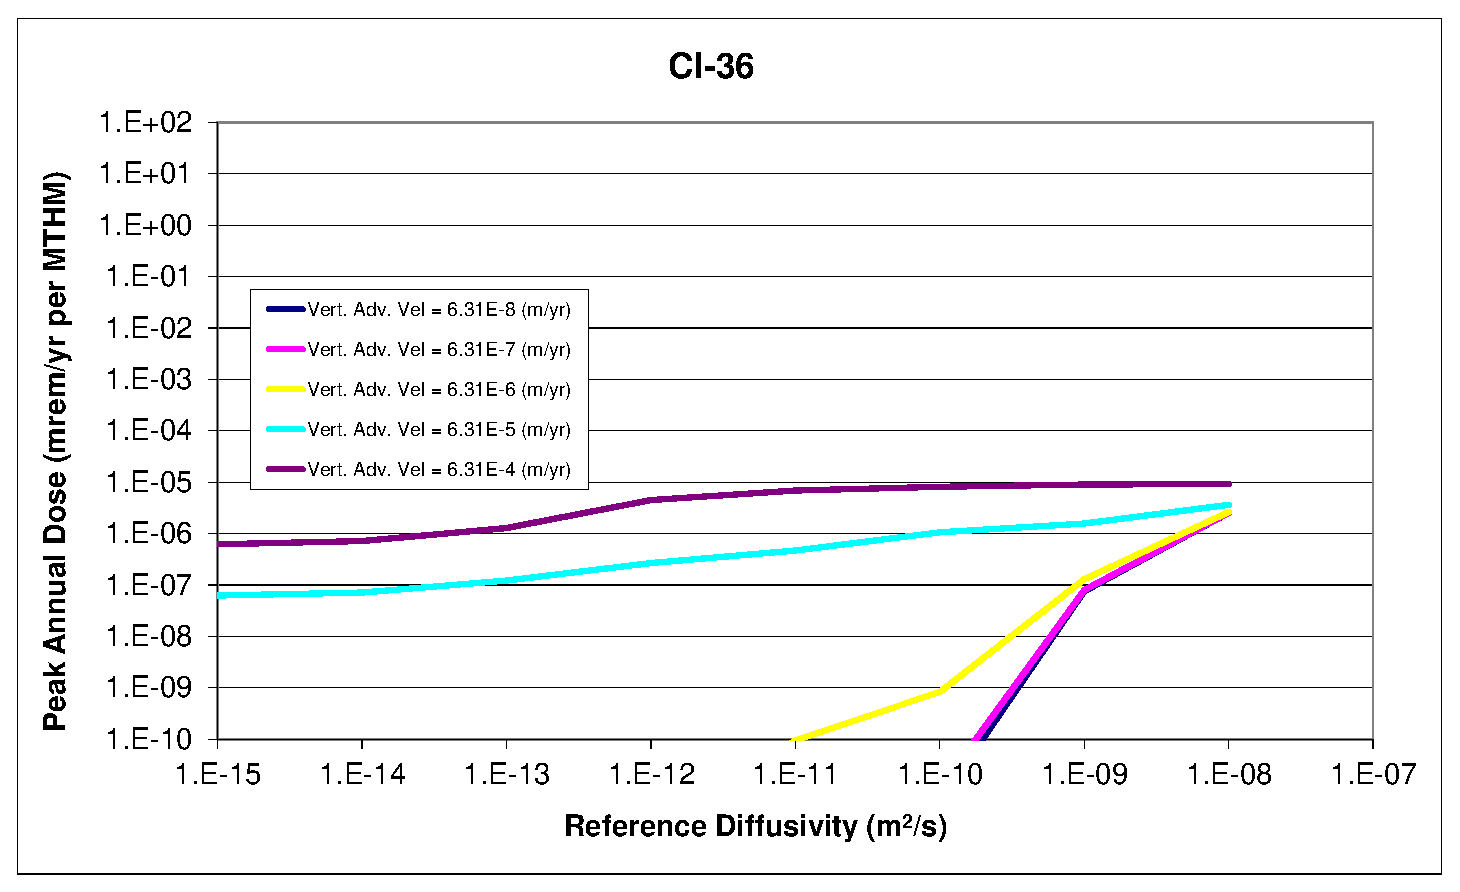
\includegraphics[width=0.8\textwidth]{AdvVelAndDiffCoeffEBSFail/Cl-36.eps}
\caption{$^{36}Cl$.
For vertical advective velocities 
$6.31\times10^{-6}[m/yr]$ and above, lower reference diffusivities are 
ineffective at attenuating the mean of the peak doses for soluble, non-sorbing 
elements. 
}
\label{fig:VAdvVelCl36}
\end{figure}
\end{frame}


\begin{frame}[c]
  \frametitle{Case II : Vertical Advective Velocity and Diffusion Coefficient}

\begin{figure}[ht!]
\centering
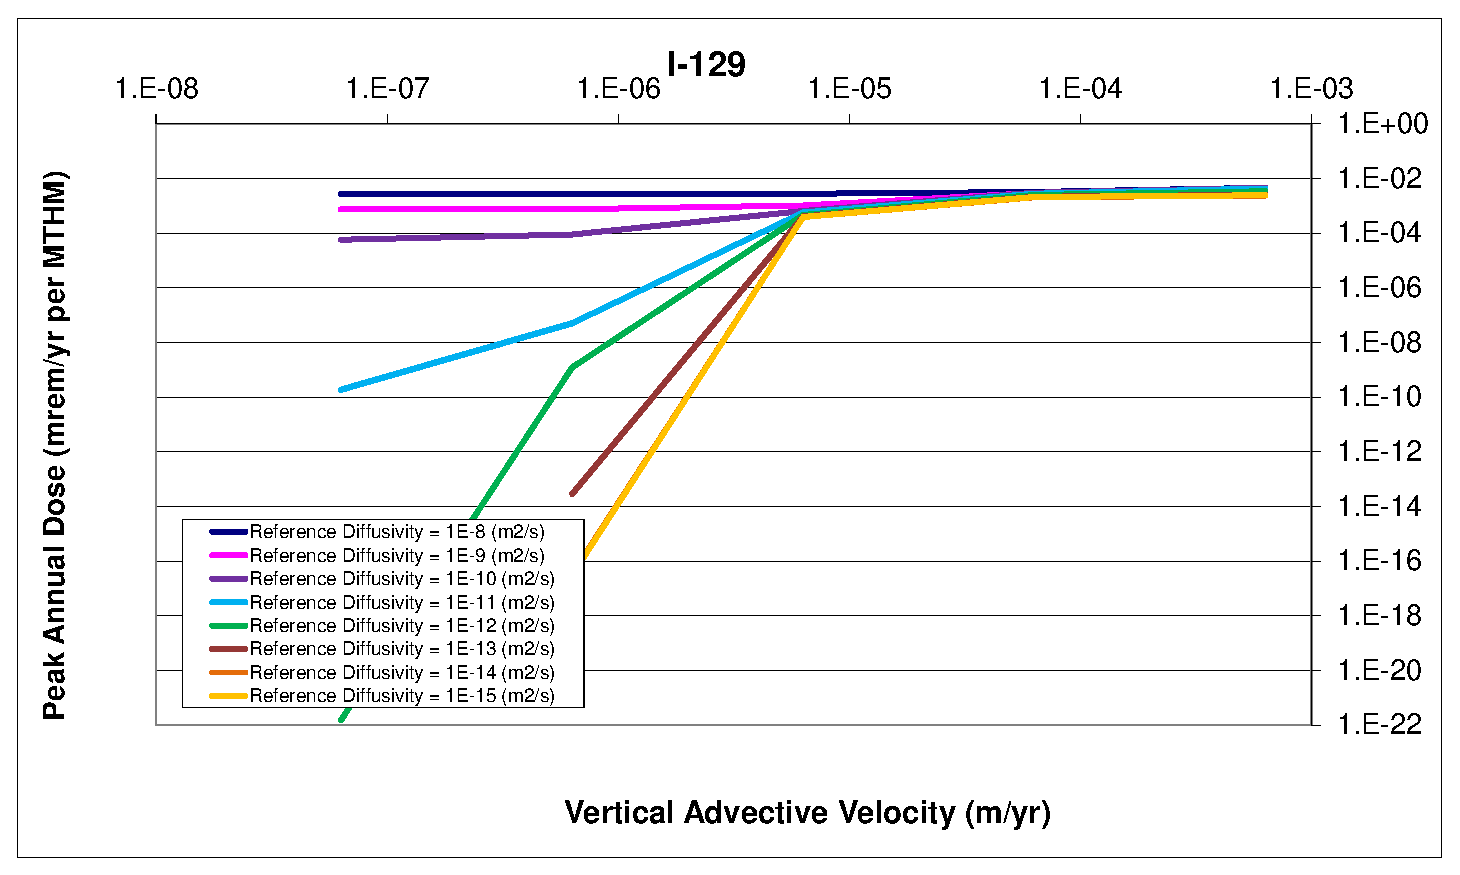
\includegraphics[width=0.8\textwidth]{AdvVelAndDiffCoeffEBSFail/I-129-VAdvVel.eps}
\caption{$^{129}I$.
For vertical advective velocities 
$6.31\times10^{-6}[m/yr]$ and above, lower reference diffusivities are 
ineffective at attenuating the mean of the peak doses for soluble, non-sorbing 
elements. 
}
\label{fig:VAdvVelI129VAdvVel}
\end{figure}
\end{frame}



\begin{frame}[c]
  \frametitle{Case II : Vertical Advective Velocity and Diffusion Coefficient}
\begin{figure}[ht!]
\centering
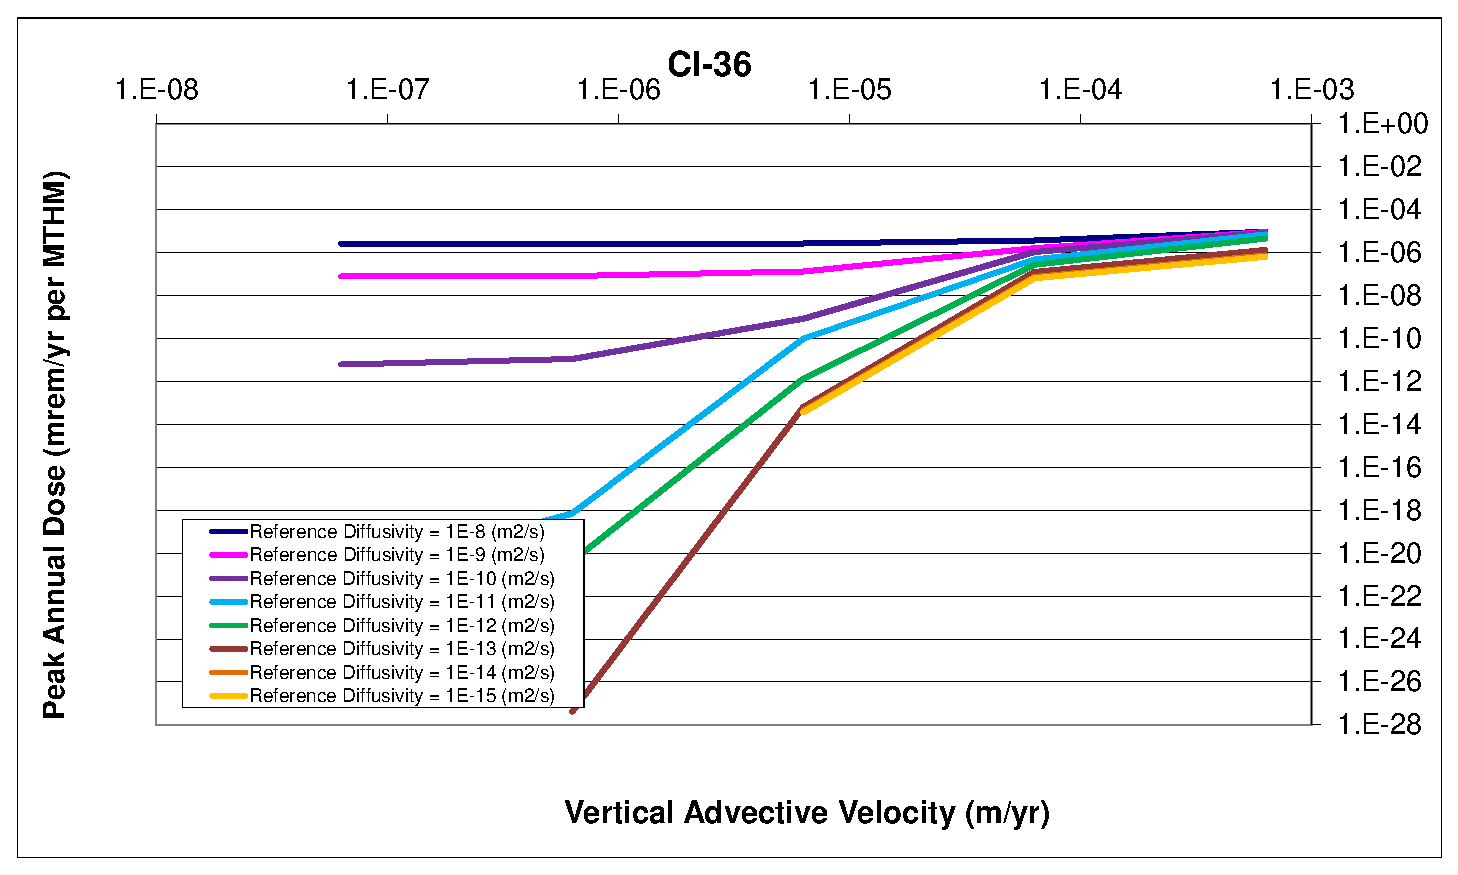
\includegraphics[width=0.8\textwidth]{AdvVelAndDiffCoeffEBSFail/Cl-36-VAdvVel.eps}
\caption{$^{36}Cl$.
For vertical advective velocities 
$6.31\times10^{-6}[m/yr]$ and above, lower reference diffusivities are 
ineffective at attenuating the mean of the peak doses for soluble, non-sorbing 
elements. 
}
\label{fig:VAdvVelCl36VAdvVel}
\end{figure}
\end{frame}

\begin{frame}[c]
  \frametitle{Case II : Vertical Advective Velocity and Diffusion Coefficient}
The solubility limited and sorbing elements, $Tc$ and $Np$, in Figures 
\ref{fig:VAdvVelTc99}, \ref{fig:VAdvVelTc99VAdvVel}, \ref{fig:VAdvVelNp237}, and 
\ref{fig:VAdvVelNp237VAdvVel}

Dose contribution from $^{99}Tc$ has a proportional 
relationship with vertical advective velocity above a regime threshold at 
$6.31\times10^{-5}[m/yr]$, above which the system exhibits sensitivity to 
advection. 

%There is an interesting feature in which $^{99}Tc$ 
%exhibits a decrease in peak annual dose for an increase in reference diffusivity 
%for the very high ($6.31\times10^{-4}$) vertcial advective velocity case. %WHY? 
\end{frame}

\begin{frame}[c]
  \frametitle{Case II : Vertical Advective Velocity and Diffusion Coefficient}
\begin{figure}[htp!]
\centering
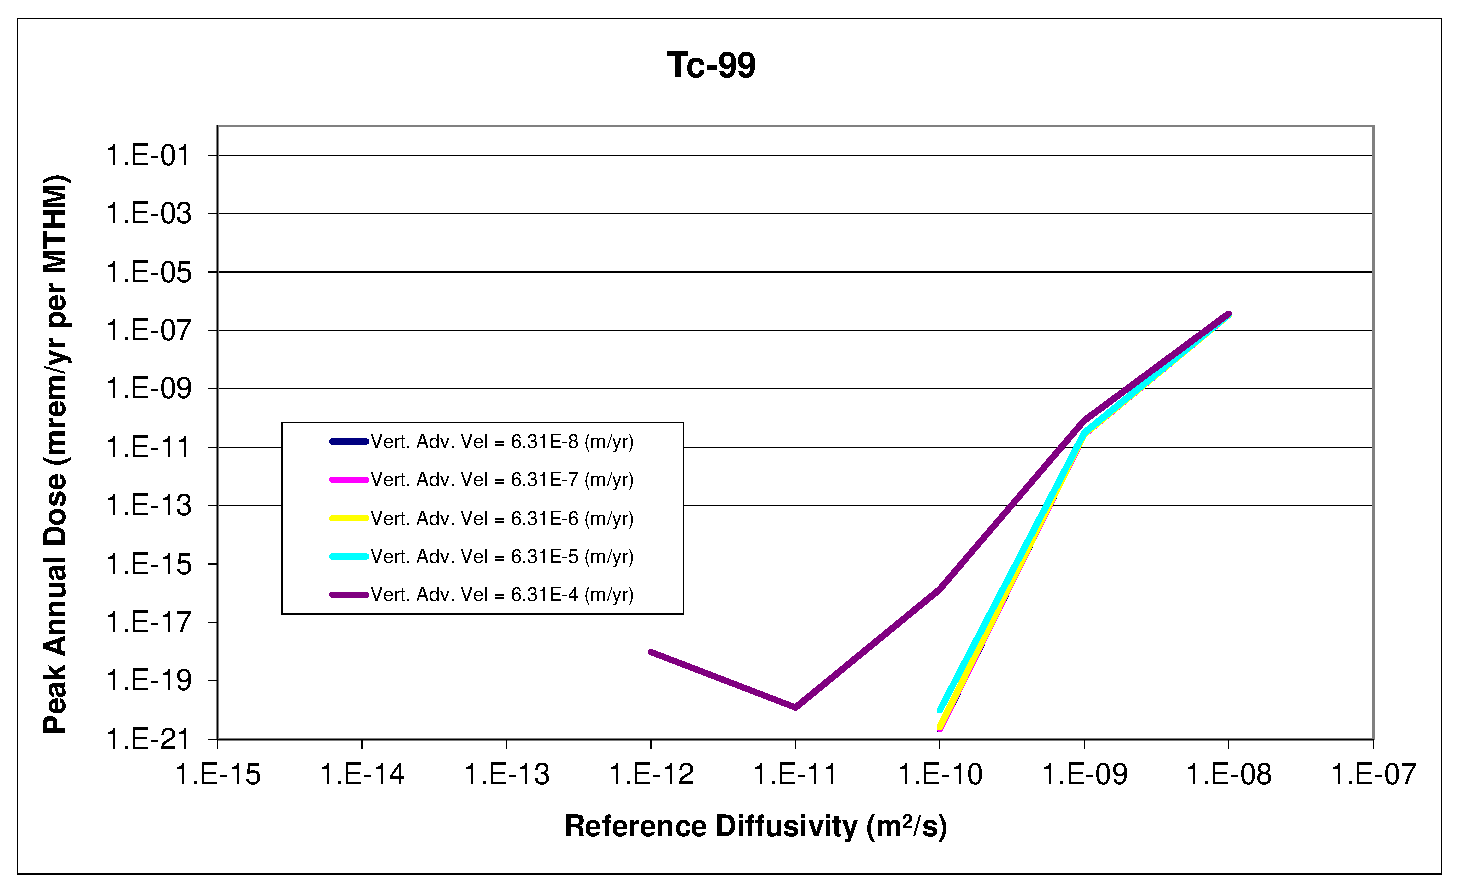
\includegraphics[width=0.8\textwidth]{AdvVelAndDiffCoeffEBSFail/Tc-99.eps}
\caption{$^{99}Tc$ 
shows a very weak influence on peak annual dose 
rate for low reference diffusivities, but a direct proportionality between 
dose and reference diffusivity above a threshold.}
\label{fig:VAdvVelTc99}
\end{figure}
\end{frame}

\begin{frame}[c]
  \frametitle{Case II : Vertical Advective Velocity and Diffusion Coefficient}
\begin{figure}[htp!]
\centering
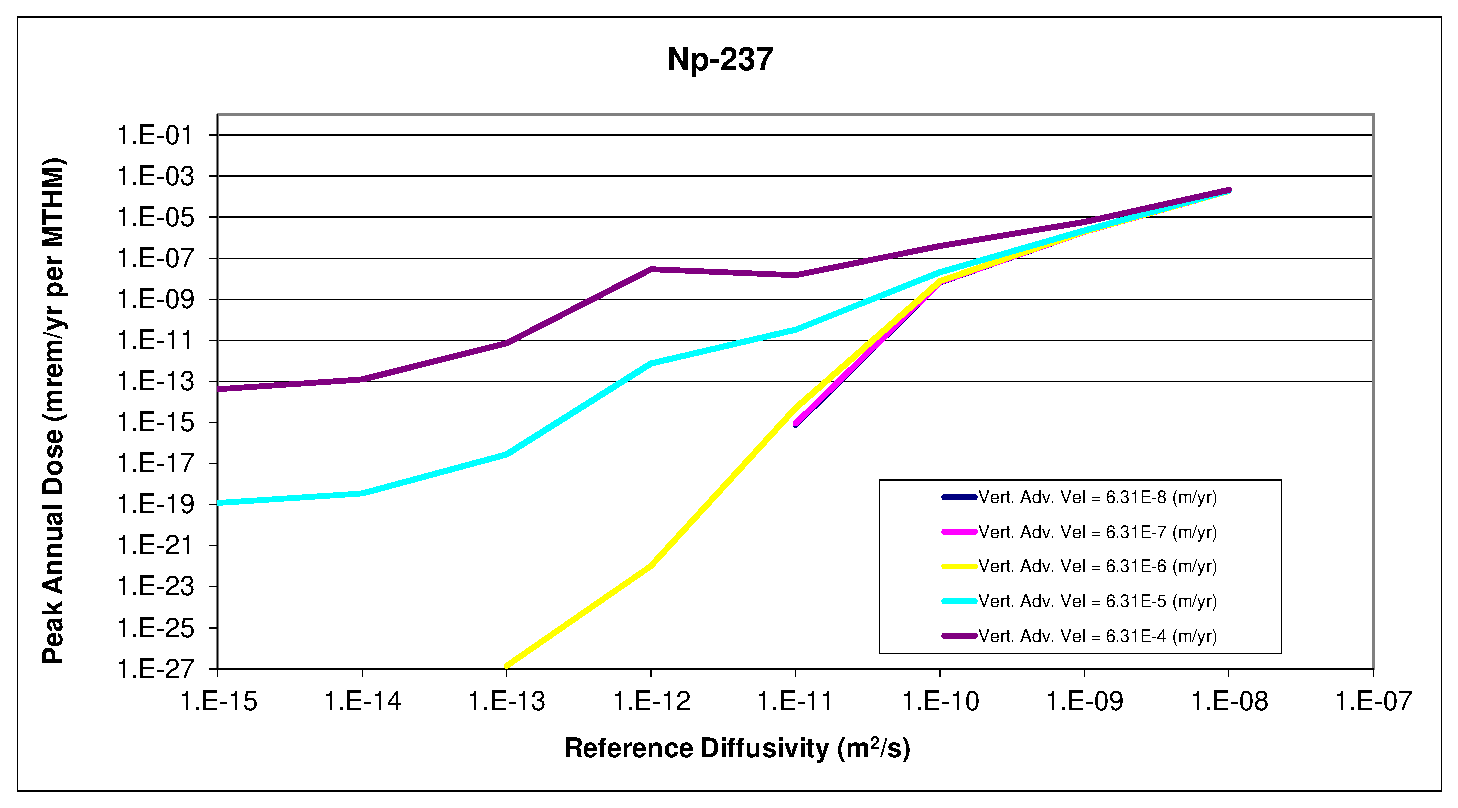
\includegraphics[width=0.8\textwidth]{AdvVelAndDiffCoeffEBSFail/Np-237.eps}
\caption{$^{237}Np$.
shows a very weak influence on peak annual dose 
rate for low reference diffusivities, but a direct proportionality between 
dose and reference diffusivity above a threshold.}
\label{fig:VAdvVelNp237}
\end{figure}
\end{frame}

\begin{frame}[c]
  \frametitle{Case II : Vertical Advective Velocity and Diffusion Coefficient}
\begin{figure}[htp!]
\centering
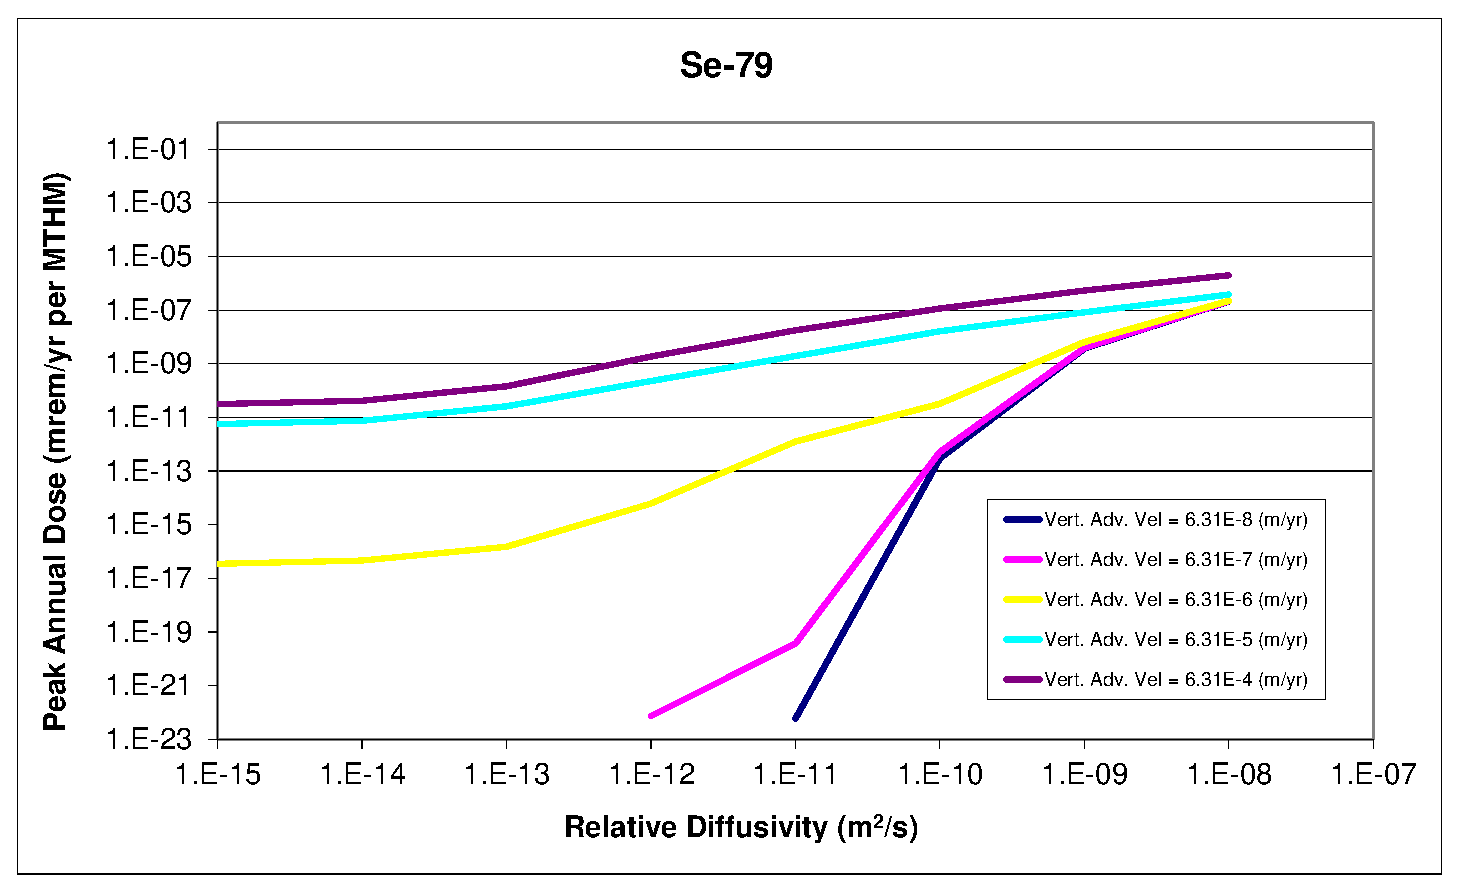
\includegraphics[width=0.8\textwidth]{AdvVelAndDiffCoeffEBSFail/Se-79.eps}
\caption{$^{79}Se$.
$Se$ is non sorbing, but solubility limited.  
For low vertical advective velocity, 
the system is diffusion dominated.}
\label{fig:VAdvVelSe79}
\end{figure}
\end{frame}


\begin{frame}[c]
  \frametitle{Case II : Vertical Advective Velocity and Diffusion Coefficient}
\begin{figure}[ht!]
\centering
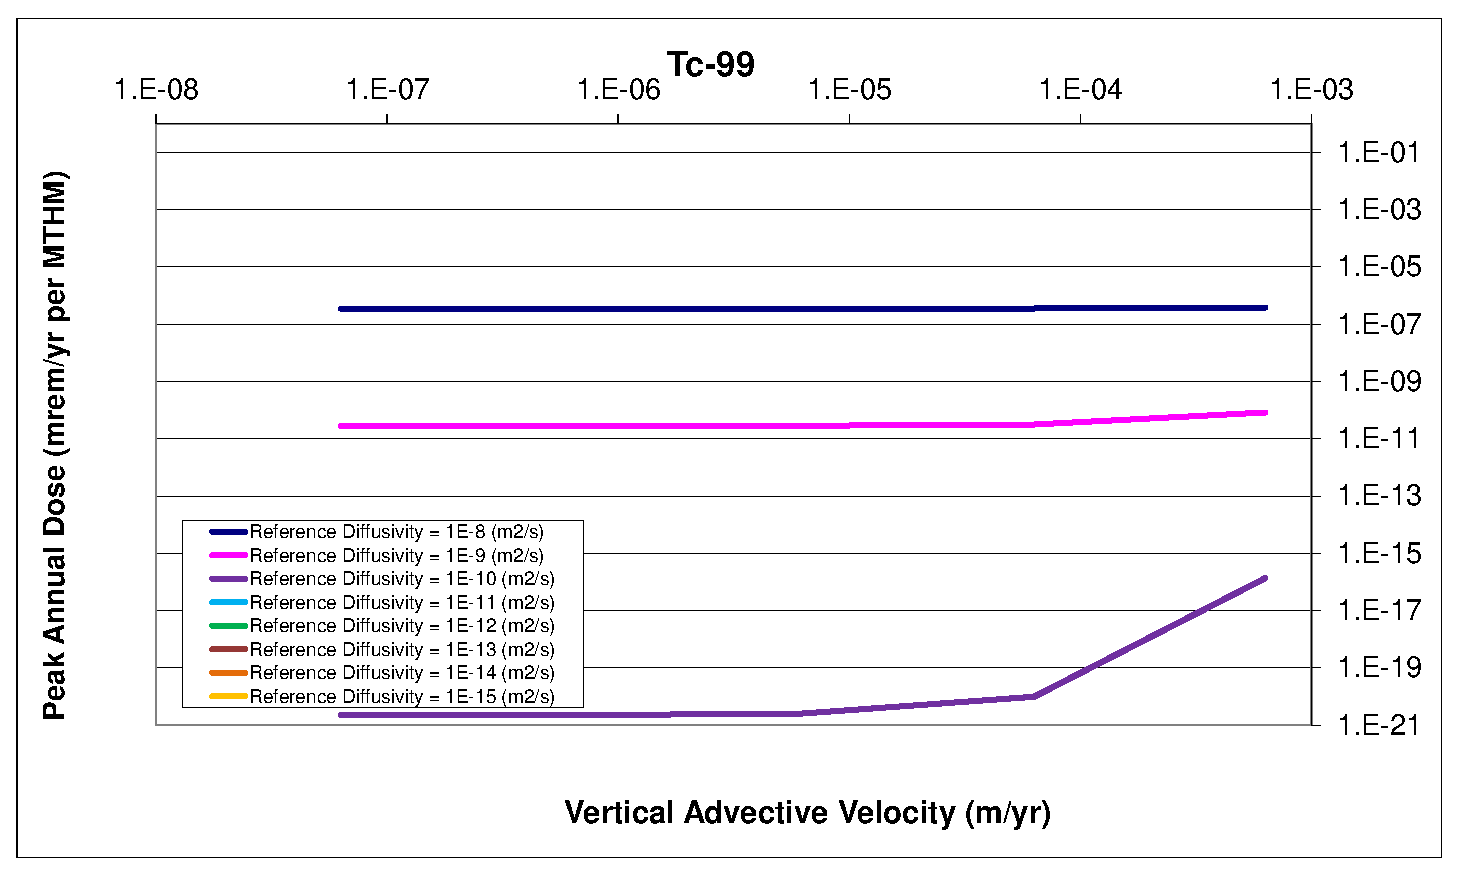
\includegraphics[width=0.8\textwidth]{AdvVelAndDiffCoeffEBSFail/Tc-99-VAdvVel.eps}
\caption{$^{99}Tc$.
shows a very weak influence on peak annual dose 
rate for low reference diffusivities, but a direct proportionality between 
dose and reference diffusivity above a threshold.}
\label{fig:VAdvVelTc99VAdvVel}
\end{figure}
\end{frame}


\begin{frame}[c]
  \frametitle{Case II : Vertical Advective Velocity and Diffusion Coefficient}
\begin{figure}[ht!]
\centering
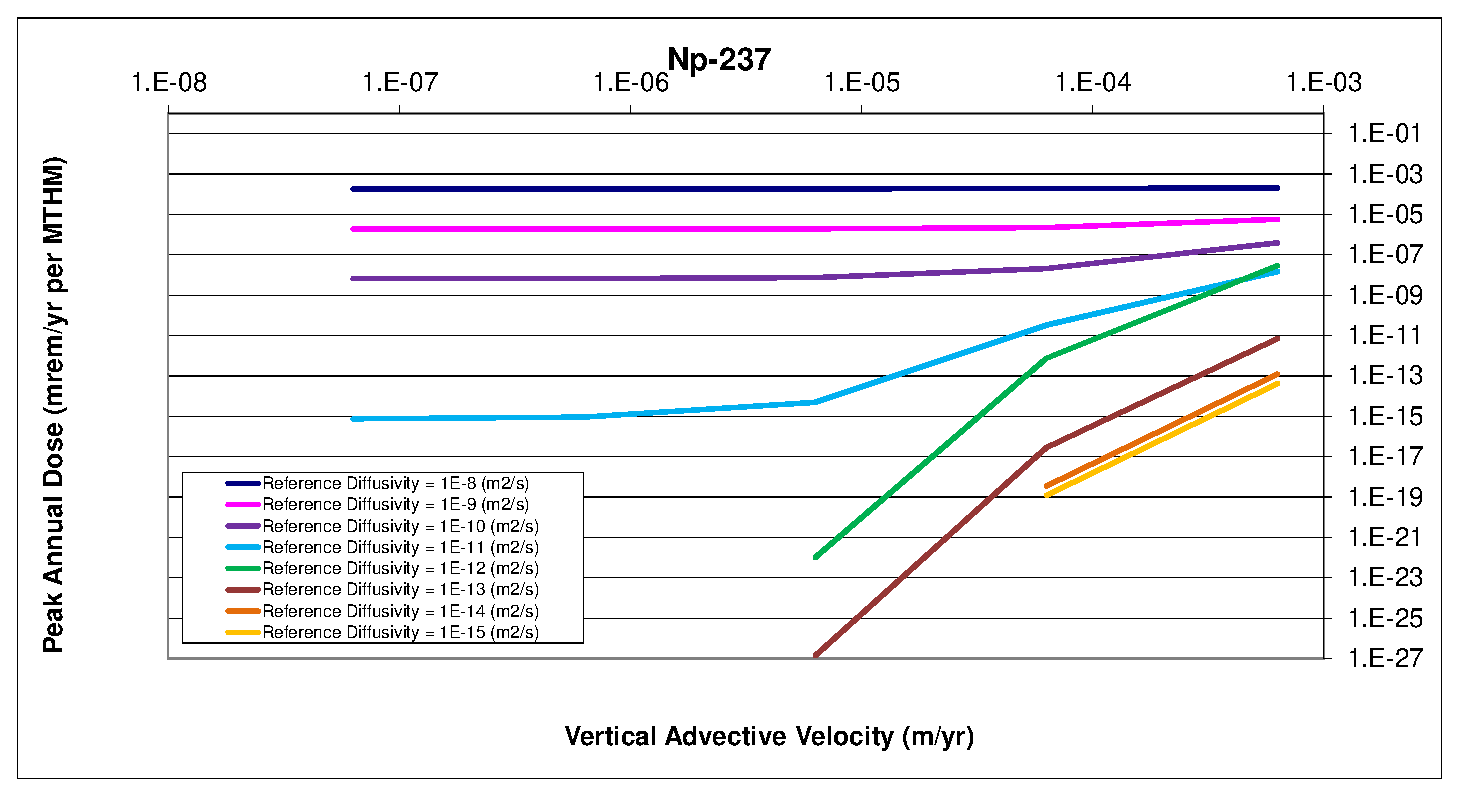
\includegraphics[width=0.8\textwidth]{AdvVelAndDiffCoeffEBSFail/Np-237-VAdvVel.eps}
\caption{$^{237}Np$.
shows a very weak influence on peak annual dose 
rate for low reference diffusivities, but a direct proportionality between 
dose and reference diffusivity above a threshold.}
\label{fig:VAdvVelNp237VAdvVel}
\end{figure}
\end{frame}

\begin{frame}[c]
  \frametitle{Case II : Vertical Advective Velocity and Diffusion Coefficient}
\begin{figure}[ht!]
\centering
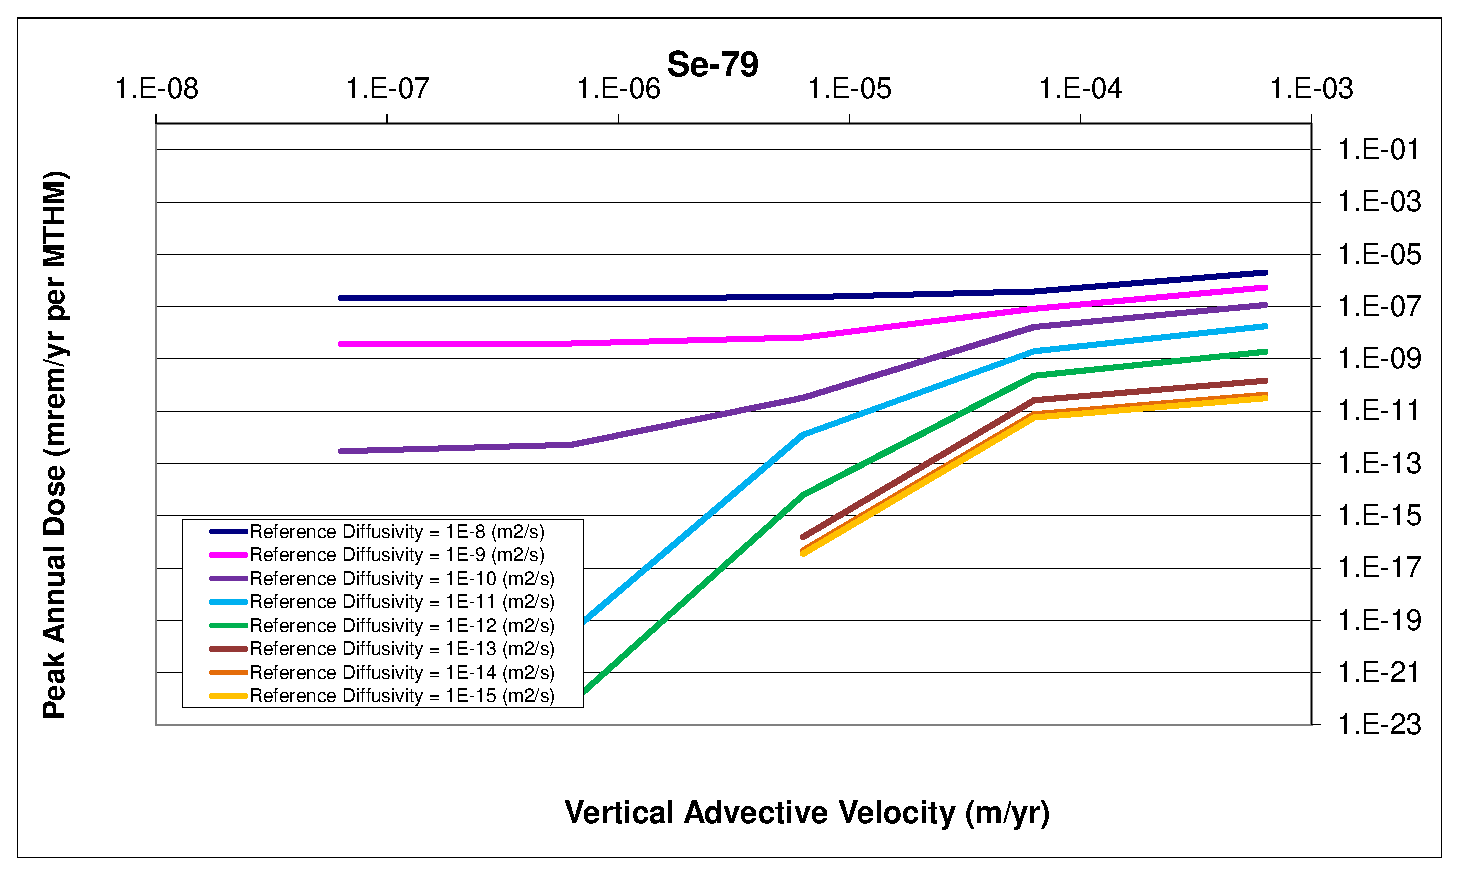
\includegraphics[width=0.8\textwidth]{AdvVelAndDiffCoeffEBSFail/Se-79-VAdvVel.eps}
\caption{$^{79}Se$.
$Se$ is non sorbing, but solubility limited.  
For high vertical advective 
velocity, the diffusivity remains important even in the advective regime as 
spreading facilitates transport in the presence of solubility limited transport. 
vertical advective velocity sensitivity.}
\label{fig:VAdvVelSe79VAdvVel}
\end{figure}
\end{frame}

